% !TeX root = ../main-paper.tex
\section{Experiment 2: Impact of OCR nosie on named entity recognition}
\label{sec:ner-xp2}
Noise introduced by OCR is known to impede the named entity recognition process (see section~\ref{subsection:stoa-ner-on-historical-texts}).
%The second experiment assesses the impact of the OCR on the quality of the NER results.
The second experiment addresses two questions (1) which model is the most robust to OCR noise and (2) what is the most appropriate strategy to fine-tune the NER layer if the input texts to label are noisy ?

\subsection{Dataset}

To this end, we leverage the labeled OCR datasets produced following to the method explained in Section 5, in addition to the gold reference.

First and foremost, to make sure that the datasets contain the same entries a preprocessing step must be performed.
Indeed, entries where the OCR produced an empty string and those for which no entity could be projected from the gold reference text are ignored.
To overcome this problem we filter each dataset by keeping only the entries common to all.
At the cost of losing  5\% of the gold references entries, we thus have four new annotated datasets containing the exact same entries.
They are denoted hereafter {reference, pero, tesseract}-gold.
Finally each is is split into a training, a dev and a test subset following the procedure presented in\cref{subsection:experiment-1-setup}.



\subsection{Metrics}
prec/recall/F1 as in \ref{sec:ner-xp1}

The whole process is illustrated on~\cref{fig.eval-ocr-ner}. The OCR text and the GOLD text are first aligned to
evaluate the OCR accuracy. As there are 11 mismatches over 56 aligned characters, the CER is thus 24\%. This alignment
is then used to back-project the GOLD tags to build the tagged NER reference string. Finally, the NER system runs on the
OCR text; its output is compared to the NER reference string. There is only 2 over 3 tags matching in the prediction (precision),
while only 2 over 4 entities are matched in the reference (recall). It follows an overall f-score of 0.4.

\begin{figure}[tb]
    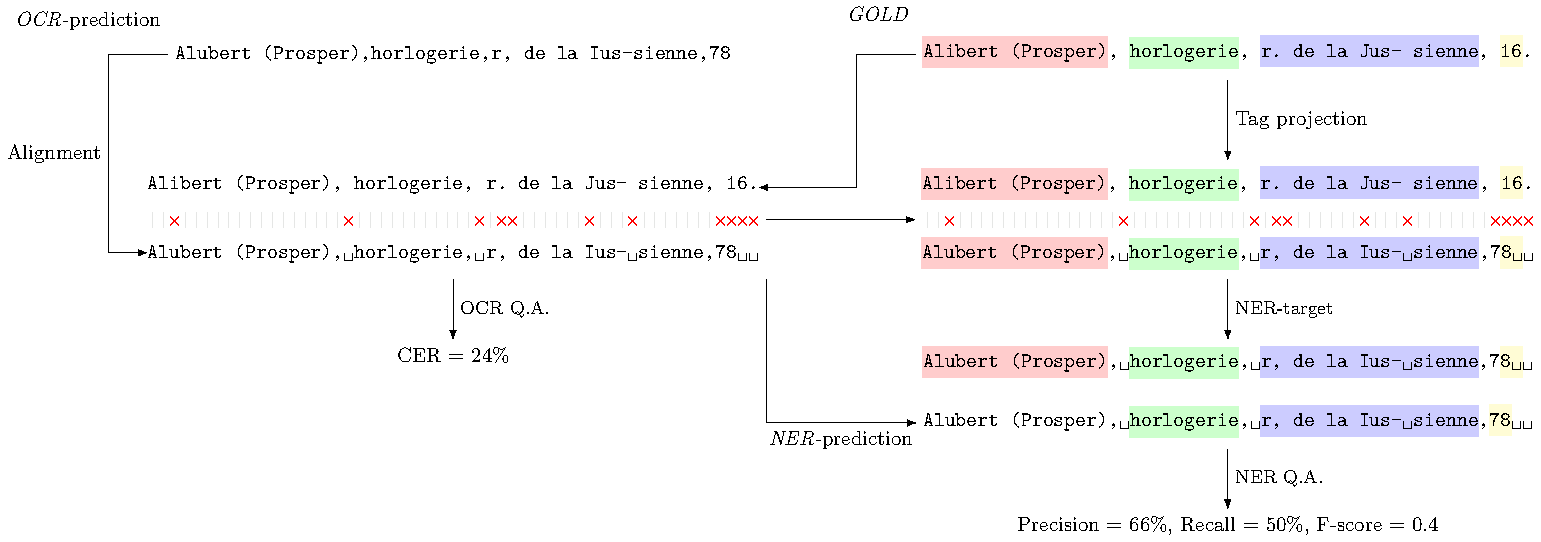
\includegraphics[width=\linewidth]{figs/eval-ocr-ner.pdf}
    \caption{OCR and NER evaluation protocol example.}
    \label{fig.eval-ocr-ner}
\end{figure}



\subsection{Systems/Variants under test}


\subsubsection{Huggingface CamemBERT}
\joseph{Copie de \cref{sub:ner-xp1-sysytems-huggingcam}. Je suggère de rédiger la section de l'XP 1 en premier et apporter précision nécessaires ici.}

Experiments 1 and 2 rely on the implementation of transformers provided by the software library Huggingface (transformers v.4.15.0, datasets v.1.17.0).
Our baseline CmBERT model is CamemBERT model published on the Hugging Face repository \footnote{\url{https://huggingface.co/Jean-Baptiste/camembert-ner}} and already trained for NER on wikiner-fr.
Its NER head is a linear model with a Softmax function.
CmBERT and CmBERT+ptrn are always fine-tuned using the same parameters, with at most 5000 training steps and an early stopping condition set to 3 evaluations in experiment 1 (5 in experiment 2) without improvement of the f1 score. Evaluations are performed every 100 steps.

\subsection{Protocol}

We fine-tune CmBERT and CmBERT+ptrn on reference-gold and pero-gold to create two versions of each model: the former trained on manually corrected entries and the latter on OCR entries.
SpaCy NER is left aside as results from experiment 1 show that it is outperformed by BERT models.
Performance metrics are computed for each of the four resulting NER models against the test sets created from reference-gold, pero-gold and tesseract-gold.


\subsection{Results and discussion}


CmBERT and CmBERT+ptrn are fine-tuned on the training sets from reference-gold (manually corrected entries) and pero-gold to produce 4 different models.
Their F1 score measured against the test tests from reference-gold, pero-gold and tesseract-gold are given in \cref{fig:exp_2_eval_ner}.
The results clearly show that models perform best when both the pre-training and the NER fine-tuning share the same characteristics (here, OCR noise) as the texts to be processed.

In our tests, pre-training the model brings a slight gain in performance ($\approx 0.5\%$).
We did not pre-train or fine-tune with texts extracted with Tesseract.
However, despite a loss of performance the model pre-trained and fine-tuned with pero-gold still gives the best results.
This is probably due to the fact that the texts produced by Pero-OCR feature characteristics intermediary between human transcriptions and Tesseract.

\begin{figure}
    \centering
    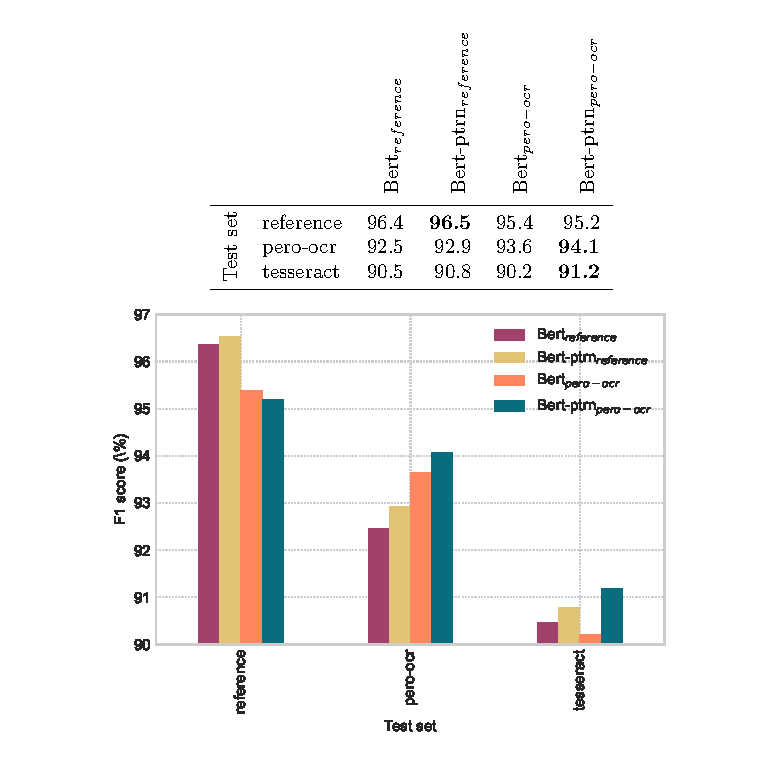
\includegraphics[width=\textwidth]{figs/eval-ner-exp2.pdf}
    \caption{F1 scores (in \%) of NER predictions in presence of OCR noise in the training and testing examples, either manually corrected or raw from Pero-OCR and Tesseract. The type of examples used to train the NER task is noted in indice after the model name (e.g. Bert$_{reference}$). Results show that best performances on OCRed entries are obtained when the BERT model has been pretrained and fine-tuned for NER on examples affected with similar OCR errors.}
    \label{fig:exp_2_eval_ner}
\end{figure}

